\section{User Tests}
\label{sec:evaluation:user-tests}

This section will describe the experimental procedures carried out during the project to determine how well it performed when used by
other people and how well it performed comparing to the requirements specified in \Cref{sec:requirements-specification}.

\subsection{Goal}

\subsection{Setup}
\label{sec:evaluation:user-tests-setup}

The setup of our user test consisted of a Macbook Pro running OpenHAB and Spotify, two Philips Hue lamps and two Estimote beacons.
Seven people were asked to train four unique gestures, creating ten templates per gesture resulting in a total of 40 gesture templates per person.
The gestures used were:

\begin{itemize}
  \item Circle
  \item Swipe Left to Right
  \item V
  \item Zorro
\end{itemize}

The setup was limited to a subset of the smart devices and gestures presented in the scenario in \Cref{sec:analysis:scenarios}, because we did not have the necessary hardware and space available to perform a test of the entire scenario as well as to keep the invested time for each participant to a minimum, so it is more likely that they could schedule time to participate in a test.

\begin{figure}[h]
\centering
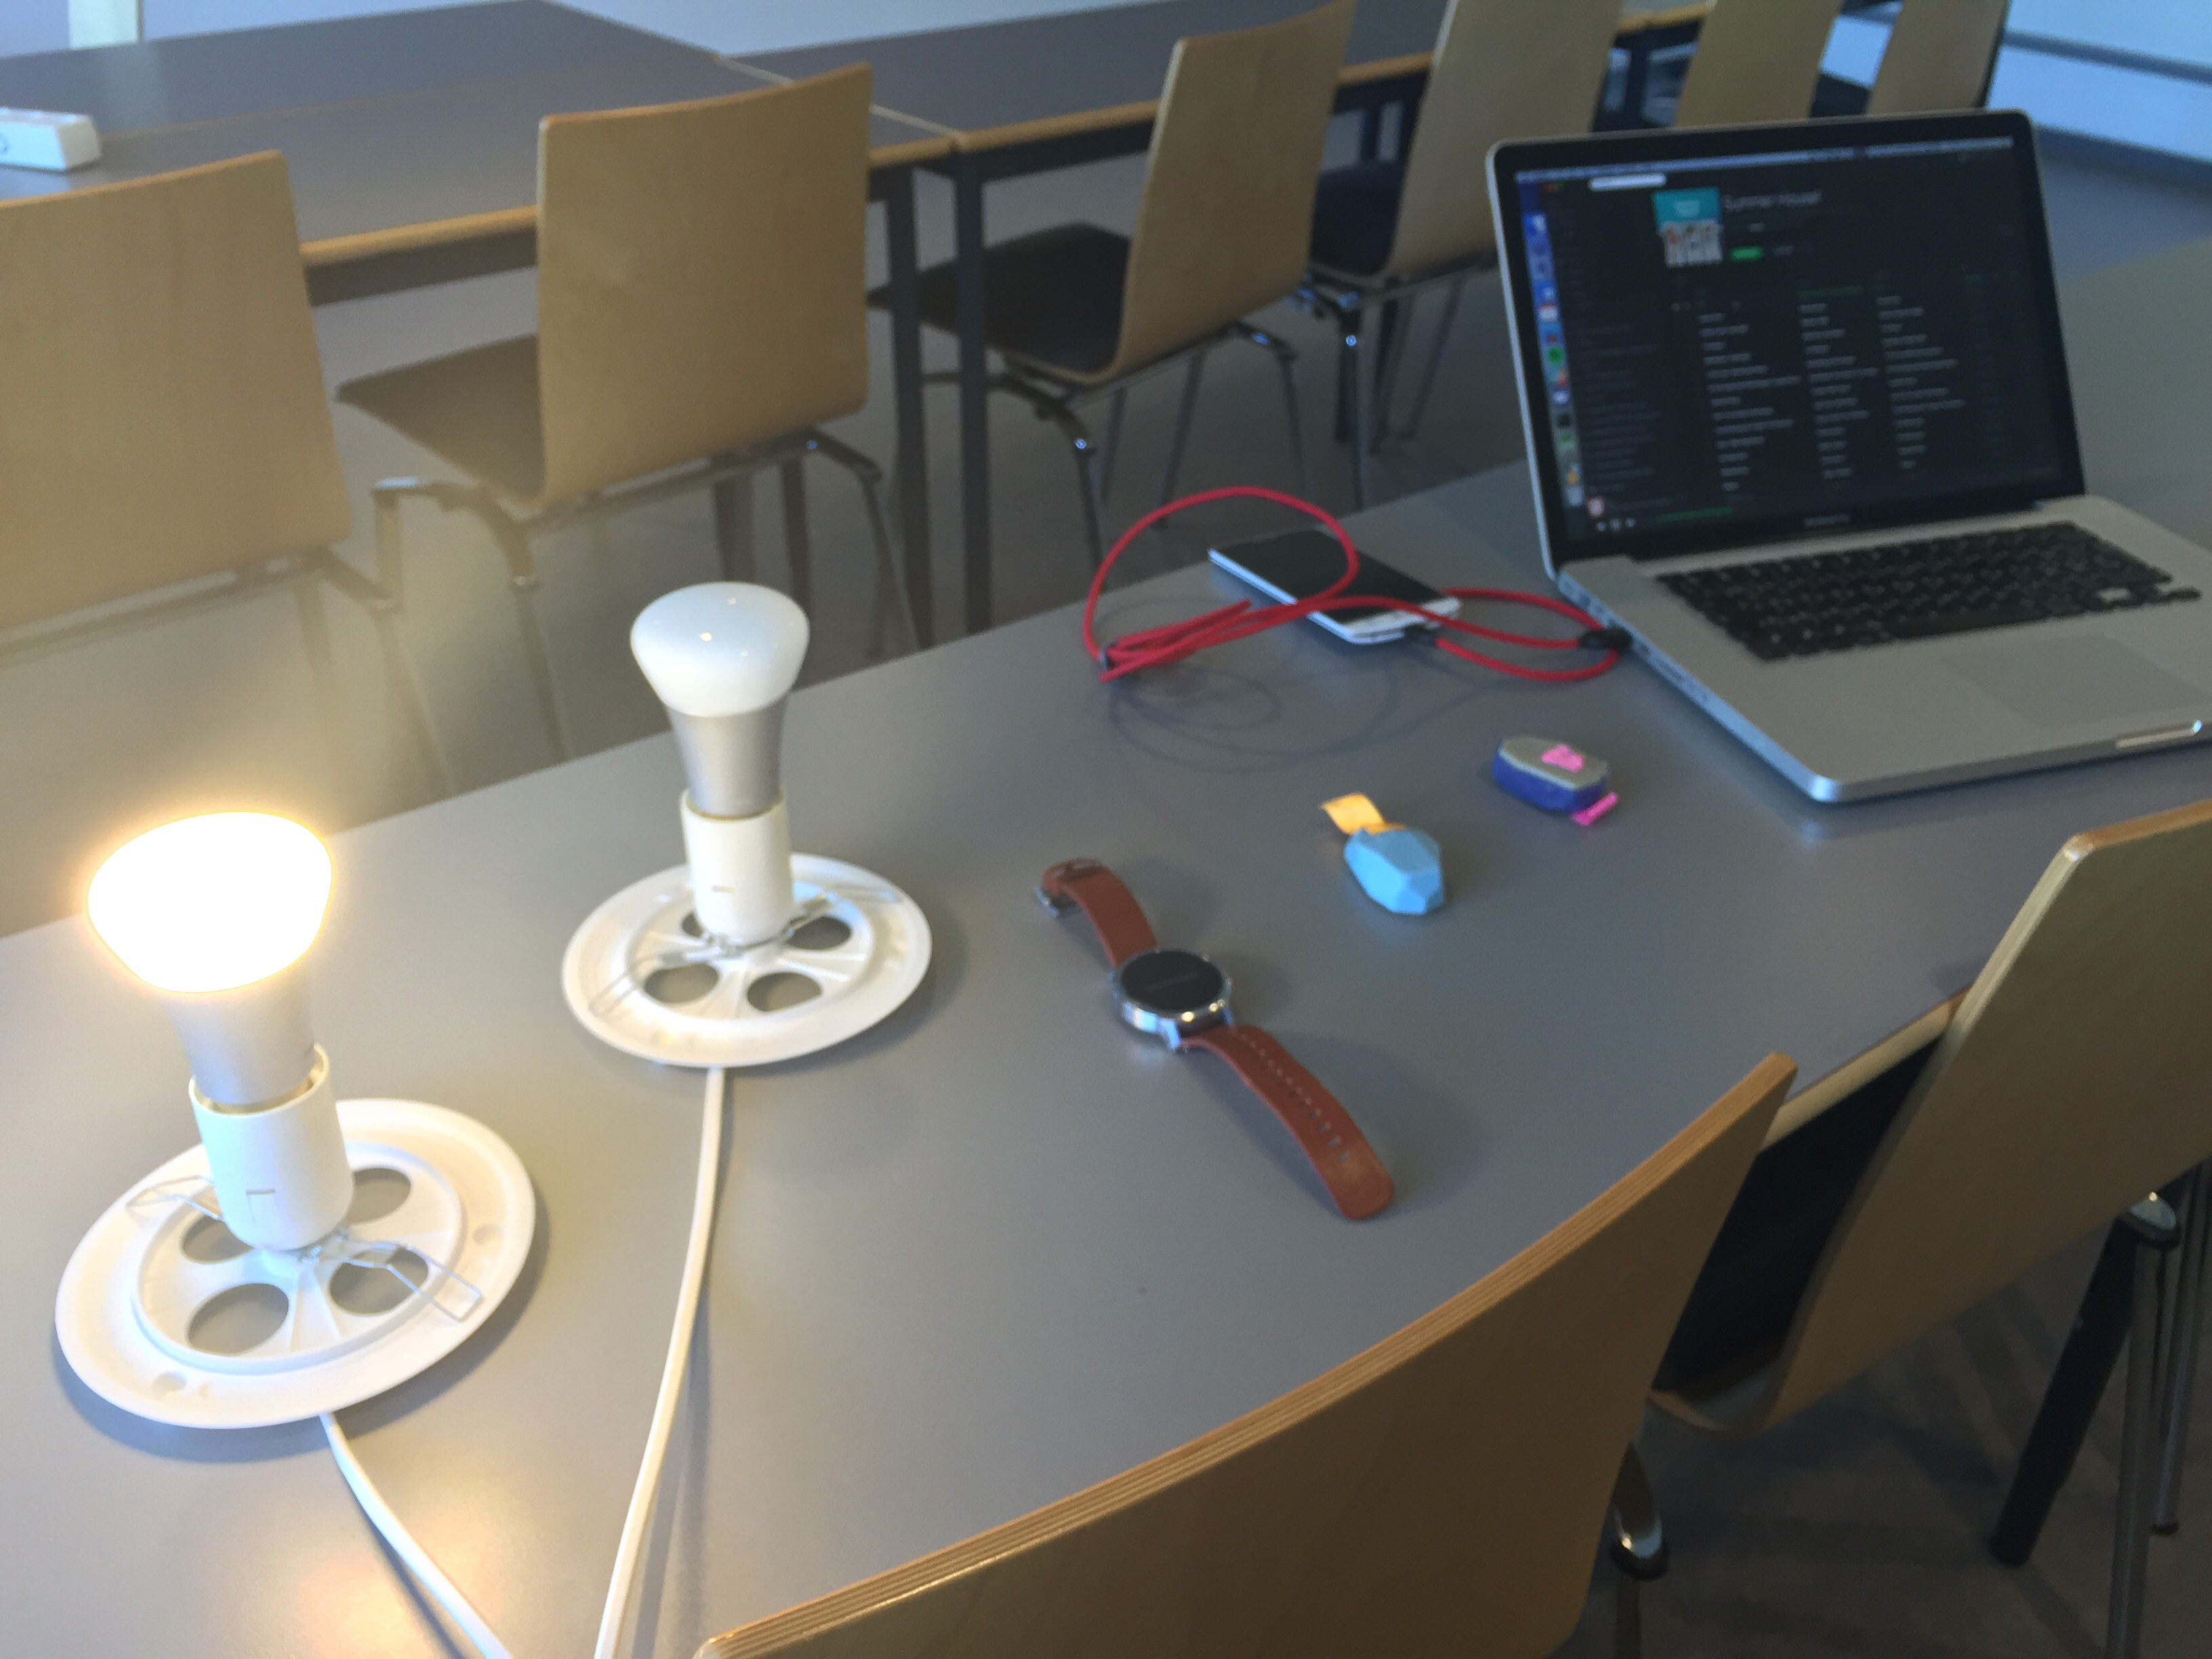
\includegraphics[width=0.45\textwidth]{images/user-test-setup.jpg}
\caption{Image of the setup used for the user tests.}
\label{fig:user-test-setup-image}
\end{figure}

The gesture templates stored in the database were removed before each test so each participant was only using his own templates and not those created by others.

The participants were instructed how to perform the gestures but were allowed to scale them to their personal preference, \eg either create large circles or small circles.

\subsection{Method}

Once the gesture templates had been created the participants were asked to complete seven tasks, each of which required them to perform a given gesture five times.
Tests took place in a single room but to simulate the user moving between two different rooms, only one Estimote beacon would be turned on at a time.
A list of the gestures and locations is shown in in \Cref{table:user-test-tasks}, along with the OpenHAB actions they were supposed to trigger.

\begin{table}[h]
\centering
\begin{tabular}{|l|l|l|}
\hline
\textbf{Action}         & \textbf{Gesture}    & \textbf{Location}              \\ \hline
Shelves\_Lamp\_Toggle   & V                   & Home Office                    \\ \hline
Spotify\_PlayPause      & Circle              & Home Office                    \\ \hline
Spotify\_Next           & Swipe Left to Right & Home Office                    \\ \hline
Architect\_Lamp\_Toggle & V                   & Living Room                    \\ \hline
TV\_Lamp\_Toggle        & Zorro               & Living Room                    \\ \hline
Spotify\_Next           & Swipe Left to Right & Home Office (Virtual Position) \\ \hline
Shelves\_Lamp\_Toggle   & V                   & Home Office                    \\ \hline
\end{tabular}
\caption{The actions, gestures and locations that were used during the user tests.}
\label{table:user-test-tasks}
\end{table}

For each participant and task, the success rate of the actions triggered was calculated as the \emph{number of times the intended action was triggered} divided by the \emph{number of attempts} and can be found in \Cref{fig:user-test-action-correctness}.
In the same manner, the success rate for gestures and locations have been plotted in \Cref{fig:user-test-gesture-correctness,fig:user-test-location-correctness}.
For each participant, the average success rate for all actions, gestures, and locations can be found in \Cref{table:user-task-averages}.
\Cref{fig:participant-average} shows the combined averages of all participents separated per task.

\subsection{Results}
\label{sec:evaluation:user-tests-results}

The average success rate of actions is below the 80\% requirement specified in \Cref{sec:requirements-specification} with a combined average of 44\%.
Triggering the correct action less than half of the time is not a satisfactory result and is thus something that needs to be looked into.
The locations are correctly identified in the majority of the cases with an average success rate of 83\% which indicates that the positioning is reliable.

One source of the inaccuracy comes from the low average success rates of the gestures.
\Cref{fig:participant-average} shows that the gesture success rates are generally higher than those of actions with an average of 56\%.
However differences between the average gesture success rates of the participants are noticable.
The most noticable example is comparing \Cref{fig:participant-1,fig:participant-2}.
Something to note here is that both of these participants, as well as participant 1 experienced some technical difficulties which prevented them from completing the \emph{Spotify\_PlayPause (Virtual)} task.
Participant 2 has an average success rate for gestures of \emph{93\%} and participant 6 has an average success rate of \emph{20\%}.
This is a significant difference and indicates that possibly something went wrong during the tests of participant 6, or the gesture recognizer is not capable of handling people with different capabilities of performing these gestures.

Another source of the inaccuracy of actions is the way we have modeled the context engine.
Loking at the corectness rates for \emph{Shelves_Lamp_Toggle} in \Cref{fig:participant-1} shows that the correct gesture and location was always identified, yet the correct action was only triggered 40\% of the time.

\begin{table}[h]
\centering
\begin{tabular}{|l|l|}
\hline
\textbf{Intended Action}   & Shelves_Lamp_toggle \\ \hline
\textbf{Intended Gesture}  & V                   \\ \hline
\textbf{Intended Location} & Home_Office         \\ \hline
\textbf{Gesture}           & \textbf{Belief}     \\ \hline
Circle                     & 33.18003597         \\ \hline
Swipe Left to Right        & 0                   \\ \hline
V                          & 66.81996403         \\ \hline
Zorro                      & 0                   \\ \hline
\textbf{Gesture\_Action}   &                     \\ \hline
Spotify\_PlayPause         & 33.18003597         \\ \hline
Spotify\_Next              & 0                   \\ \hline
Shelves\_Lamp\_Toggle      & 33.40998201         \\ \hline
Architect\_Lamp\_Toggle    & 33.40998201         \\ \hline
TV\_Lamp\_Toggle           & 0                   \\ \hline
\textbf{Room}              &                     \\ \hline
Living Room                & 0                   \\ \hline
Home Office                & 100                 \\ \hline
\textbf{Room\_Action}      &                     \\ \hline
Spotify\_PlayPause         & 33.33333333         \\ \hline
Spotify\_Next              & 33.33333333         \\ \hline
Shelves\_Lamp\_Toggle      & 33.33333333         \\ \hline
Architect\_Lamp\_Toggle    & 0                   \\ \hline
TV\_Lamp\_Toggle           & 0                   \\ \hline
\textbf{Action}            &                     \\ \hline
Spotify\_PlayPause         & 33.25668465         \\ \hline
Spotify\_Next              & 16.66666667         \\ \hline
Shelves\_Lamp\_Toggle      & 33.37165767         \\ \hline
Architect\_Lamp\_Toggle    & 16.70499101         \\ \hline
TV\_Lamp\_Toggle           & 0                   \\ \hline
\end{tabular}
\caption{Belief values for the different nodes in the bayesian network of the context engine for a single trial of Participant 2.}
\label{table:participant-2-first-run}
\end{table}

In a single trial of participant 2 the scores in \Cref{table:participant-2-first-run} were recorded.
The gesture \emph{V} correctly received the highest belief in the \emph{Gesture} node but because \emph{V} is configured to be used with two actions, \emph{Shelves\_Lamp\_Toggle} as well as \emph{Architect\_Lamp\_Toggle}, the \emph{Gesture\_Action} node divides the belief amongst these.
The  gesture \emph{Circle} did not match as well as \emph{V} and only recieved approximately half of the belief value of \emph{V}.
However, since \emph{Circle} is only configured to trigger a single action, its belief value remains intact in the \emph{Gesture\_Action} node.
This results in the beliefs of \emph{Spotify\_PlayPause} and \emph{Shelves\_Lamp\_Toggle} being approximately equivalent even after the location beliefs have been applied.

As such it is more difficult to properly trigger actions where the gesture is configured to other actions as well, than triggering actions where the gesture is only configured for that one.

As such it is easier to trigger actions that only have a single gesture associated with them than actions that have multiple.

\begin{figure}[]
\begin{subfigure}{0.45\textwidth}
  \begin{tikzpicture}
  \begin{axis}[
    ybar,
    bar width=2pt,
    xticklabels from table={data/ActionCorrectnessTransposed.csv}{Action},
    xtick=data,
    x tick label style={
    rotate=45,
    anchor=east,
    },
    width=0.95\textwidth,
    ymin = 0,
    ymax = 1,
    ylabel = success rate
    ]
    \addplot table[x=Row, y=2] {data/GestureCorrectness.csv};
    \addplot table[x=Row, y=2] {data/ActionCorrectnessTransposed.csv};
    \addplot table[x=Row, y=2] {data/LocationCorrectness.csv};
  \end{axis}
  \end{tikzpicture}
\subcaption{Participant 2.}
\label{fig:participant-1}
\end{subfigure}
\begin{subfigure}{0.45\textwidth}
  \begin{tikzpicture}
  \begin{axis}[
    ybar,
    bar width=2pt,
    xticklabels from table={data/ActionCorrectnessTransposed.csv}{Action},
    xtick=data,
    x tick label style={
    rotate=45,
    anchor=east,
    },
    width=0.95\textwidth,
    ymin = 0,
    ymax = 1,
    legend style={
    at={(0,0)},
    anchor=west, at={(axis description cs:1,0.5)}}]
    \addplot table[x=Row, y=6] {data/GestureCorrectness.csv};
    \addplot table[x=Row, y=6] {data/ActionCorrectnessTransposed.csv};
    \addplot table[x=Row, y=6] {data/LocationCorrectness.csv};
    \legend{Gesture, Action, Location};
  \end{axis}
  \end{tikzpicture}
\subcaption{Participant 6.}
\label{fig:participant-2}
\end{subfigure}
\caption{Average success rate for gestures, actions and locations for the participants who performed the best and worst respectively.}
\end{figure}

\begin{figure}[h]
\centering
\begin{tikzpicture}
\begin{axis}[
    ybar,
    bar width=2pt,
    xticklabels from table={data/ActionCorrectnessTransposed.csv}{Action},
    xtick=data,
    x tick label style={
    rotate=45,
    anchor=east,
    },
    width=0.42\textwidth,
    ymin = 0,
    ymax = 1,
    ylabel = success rate,
    legend style={
    at={(0,0)},
    anchor=west, at={(axis description cs:1,0.5)}}]
    \addplot table[x=Row, y=Average] {data/GestureCorrectness.csv};
    \addplot table[x=Row, y=Average] {data/ActionCorrectnessTransposed.csv};
    \addplot table[x=Row, y=Average] {data/LocationCorrectness.csv};
    \legend{Gesture, Action, Location}
\end{axis}
\end{tikzpicture}
\caption{All participants combined.}
\end{figure}

\subsection{Conclusion}
\label{sec:evaluation:user-tests-conclusion}

From the results of the user tests we can see that the average success rate of actions falls below the 80\% stated in \Cref{sec:requirements-specification} with a value of \emph{44\%}.
The two primary causes of this is likely the low average success rate of gestures and the way the context engine is modeled.

The gesture recognition performs sufficiently well for some participants, like participant 2, but the correctness varies too much between different participants.
The success rate of the gestures could perhaps be improved if the participants had been asked to practice the gestures before training and using them.
It may also work better if the users were allowed to make up their own gestures instead of using the ones selected by us.

The success rate of the actions could be improved by using a different model as the current model favors actions that have only a single gesture associated with it, as seen the example shown in \Cref{table:participant-2-first-run}.
An alternative model could be one where the \emph{Gesture} and \emph{Room} nodes were direct parents of the \emph{Action} node and removing the \emph{Gesture\_Action} and \emph{Room\_Action} nodes.

Other alternative models are presented in \Cref{sec:evaluation-alternative-models}.


%%% Local Variables:
%%% mode: latex
%%% TeX-master: "../../master"
%%% End:
